%!TEX root = ../thesis.tex

\section{本章の概要}

% 本章では,1章で述べたようにロボットの行動を考慮した歩行者の軌道予測を行う手法を提案する.歩行者の軌道予測に関する問題設定を3.2節,学習に用いたネットワーク構造を3.3章,ロボットの行動を考慮した軌道予測する方法を3.4章,ネットワークの学習方法を3.5章,及び学習環境を3.6章,ネットワークの予備実験の内容を3.7章でそれぞれ述べる.

本章では,ロボットの行動を考慮した歩行者の軌道予測手法を提案し,その詳細を述べる.まず,問題設定として歩行者のグラフ表現と軌道予測タスクの定義を行う.次に,提案手法で用いるエンコーダ・デコーダ構造のネットワークについて説明する.さらに,ロボットの行動を考慮した軌道予測の方法を示し,学習方法と学習環境についても述べる.最後に,ネットワークの基本性能を確認する.

% 以下では,予測を行うネットワーク構造とその学習方法に関して説明する.

% 〜について目指す.〜について提案する.

\section{問題設定}
本論文における歩行者のグラフ表現を説明する.まず,時刻$t$におけるシーン内の歩行者の位置を表す空間グラフを
\begin{equation}
  G_t = (V_t, E_t)
\end{equation}
と定義する.グラフ$G_t$のノードの集合を
\begin{equation}
  V_t = \{ v^i_t \mid i = 1, \dots N \}
\end{equation}
と表す.各ノード$v^i_t$は歩行者$i$の位置$(x^i_t, y^i_t)$を属性として持つ.一方,グラフ$G_t$のエッジの集合を
\begin{equation}
  E_t = \{ e^{ij}_t \mid i, j = 1, \dots N \}
\end{equation}
と表す.ノード$v^i_t$と$v^j_t$が接続されている場合に$e^{ij}_t=1$となり,そうでない場合$e^{ij}_t=0$となる.

本論文における軌道予測タスクとは,過去の観測情報をもとに,将来の歩行者の位置($x,y$座標)を予測ステップ分出力することである.
歩行者$i$の各時刻の位置を
\begin{equation}
  V_t = \{ v^i_t = (x^i_t, y^i_t) \in \mathbb{R}^2 \mid i = 1, \dots N \}
\end{equation}
と表す.また,観測時間$t_{obs}$において得られた全ての歩行者の位置データを
\begin{equation}
  V_{obs} = \{ V_t \mid t = 1, \dots t_{obs} \}  
\end{equation}
とする.ここで,時刻$t$の歩行者$i$の位置の確率分布を
\begin{equation}
  \hat{V}_t = \{ \hat{p}^i_t = (\hat{x}^i_t, \hat{y}^i_t) \mid i = 1, \dots N \} \label{hat-pos}
\end{equation}
と表す.そうすると,予測時間$t_{pred}$にわたって予測される全ての歩行者の位置データを
\begin{equation}
  V_{pred} = \{ \hat{V}_t \mid t = t_{obs + 1}, \dots t_{pred} \}
\end{equation}
と表すことができる.また,$p^i_t$が2次元正規分布$\mathcal{N}(\mu^i_t, \sigma^i_t, \rho^i_t)$に従うと仮定する.すなわち,
\begin{equation}
  \hat{p}^i_t \sim \mathcal{N}(\hat{\mu}^i_t, \hat{\sigma}^i_t, \hat{\rho}^i_t)
\end{equation}
を満たすものとする.ここで,平均は$\hat{\mu}^i_t = (\hat{\mu}^i_{x, t}, \hat{\mu}^i_{y, t})$,分散は$\hat{\sigma}^i_t = (\hat{\sigma}^i_{x, t}, \hat{\sigma}^i_{y, t})$,相関係数は$\hat{\rho}^i_t$である.これらを後述するネットワークの出力とする.

\section{ネットワーク構造}
本手法で用いるネットワークは,エンコーダ・デコーダ構造で構成されている.ネットワークは,主にエンコーダモジュール,グラフアテンションネットワークモジュール,デコーダモジュールの3つから構成される.エンコーダモジュールでは入力データから特徴量を抽出し,グラフアテンションネットワークを用いてノード間の関係性を学習する.その後,得られた潜在表現をもとにデコーダモジュールで所定のシーケンス長にわたる予測を行う.
ネットワークの概要を\figref{Fig:network}に示す.

\begin{figure}[H]
  \centering
 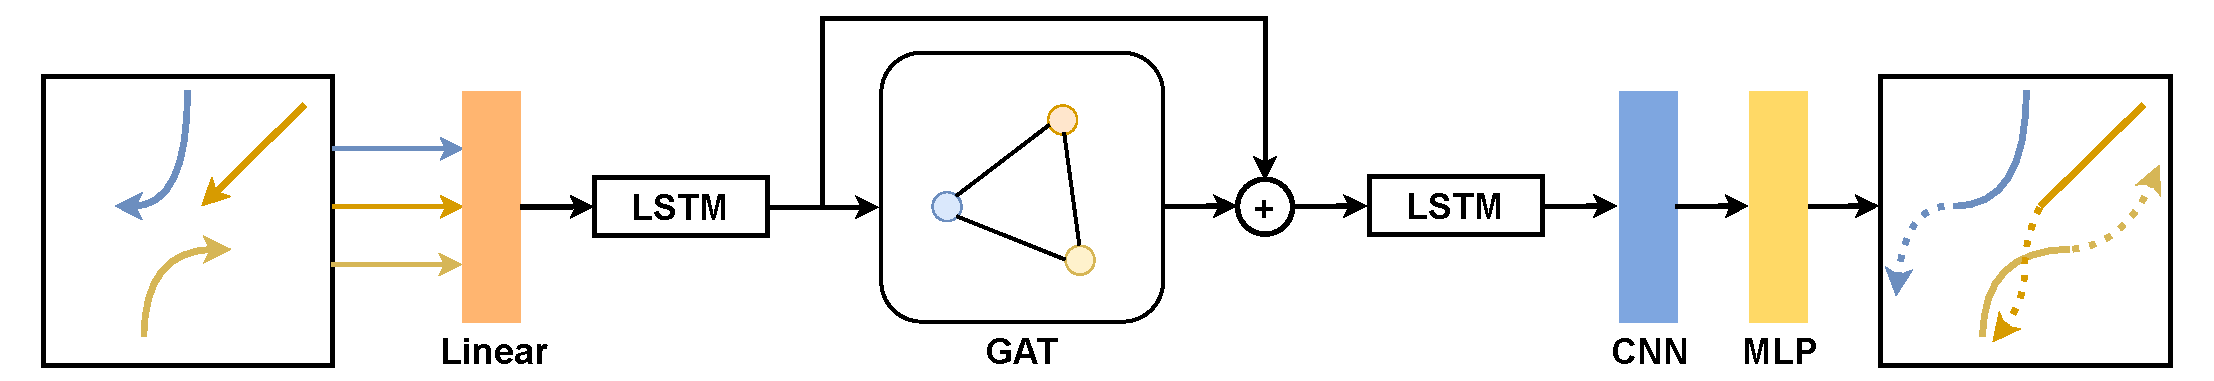
\includegraphics[keepaspectratio, scale=0.36]
      {images/network-comp.pdf}
 \caption{Network Structure}
 \label{Fig:network}
\end{figure}   

% \vspace{-20pt}

\subsection{エンコーダモジュール}
エンコーダでは,まず各時刻における歩行者の過去位置を線形変換層$\phi_{emb}$によって高次元空間へ埋め込む.この埋め込み表現をLSTM層に入力し,歩行者の過去の軌跡を時間的に処理した隠れ状態を出力する.ここで得られた隠れ状態は,歩行者の過去の動きを要約した表現となり,次に続くグラフアテンションネットワークモジュールに渡される.エンコーダにおける処理を式\eqref{emb},\eqref{lstm-en}に示す.なお,$v^i_t \text{と} v^t_i$は同義とする.
\begin{align}
  e^t_i &= \phi_{emb}(v^t_i ; W_{emb}) \label{emb} \\
  h_i &= \text{LSTM}_{en}(e^t_i, h^{t-1}_i ; W_{en}) \label{lstm-en}
\end{align}

\subsection{グラフアテンションネットワーク}
本ネットワークの中核を担うグラフアテンションネットワーク(GAT)\cite{velickovic2017graph-gat}は,マルチヘッドアテンション機構を用いる複数の層で構成される.各GAT層では,近傍ノードの特徴を集約して各ノードの特徴ベクトルを更新し,ノード間の関係強度に基づいて重み付けを行う.そのため,関連性の高いノードからの情報が強調される.複数のGAT層を積み重ねることで,グラフ構造における高次の依存関係を捉えることが可能となる.また,各タイムステップで対応する隣接行列を用いてグラフ畳み込みが実行され,動的なグラフ構造の変化にも対応できる.

歩行者$i$の隠れ状態$h_i$が与えられたとき,全歩行者に対して複数のGAT層を適用する.各層は以下のように適用される.式\eqref{gat-eij}の$e_{ij}$はノード$i$に対するノード$j$の特徴の重要度を表している.$W$は重み行列,$a$は共有アテンション機構である.また,活性化関数$\sigma$として本手法ではネットワーク全体にわたりPReLU\cite{he2015delving-prelu}を採用した.

\begin{align}
  e_{ij} = a(Wh_i, Wh_j) \label{gat-eij} \\
  \alpha_{ij} = \text{softmax}_{j}(e_{ij}) \\
  h'_i = \sigma\Bigg(\sum_{j \in \mathcal{N}_i} \alpha_{ij}Wh_j \Bigg)
\end{align}

\subsection{デコーダモジュール}\label{sec:decoder}
GAT層からの出力は,デコーダモジュールによって将来の歩行者の位置に変換される.まず,2つ目のLSTM層を用いてGAT層により生成された時空間特徴表現をさらに時間方向に処理する.次に,1次元畳み込み層(CNN)を適用し,入力シーケンス長から予測シーケンス長への変換を行う.この層は,予測時間に合わせて特徴表現の次元を調整する役割を果たす.最後に,多層パーセプトロン(MLP)を用いて予測値を生成する.式\eqref{output}に示すように,本ネットワークの最終出力は5次元である.なお,$\hat{P}^t_i\text{と}\hat{P}^i_t$は同義である.
\begin{align}
  h''_i = \text{LSTM}_{dec}(h'_i, h_{deci}; W_{dec})\\
  c^t_i = \text{CNN}(h''_i; W_{cnn}) \\
  \hat{P}^t_i = \text{MLP}_{d}(c^t_i; W_{d}) \\
  \hat{P}^i_t = [\hat{\mu}^i_{x,t}, \hat{\mu}^i_{y, t}, \hat{\sigma}^i_{x, t}, \hat{\sigma}^i_{y, t}, \hat{\rho}^i_t] \label{output}
\end{align}

さらに,本ネットワークでは\figref{Fig:network}に示すように,GAT層とLSTM層の出力に対してスキップ接続\cite{he2016deep-resnet}を導入することで,勾配消失問題\cite{hochreiter2001gradient-grad,weinleindiplomarbeit-grad, schmidhuber2015deep-grad}を軽減し,学習を安定化させる.本アーキテクチャにより,時系列データの動的な変化とグラフ構造におけるノード間の複雑な依存関係を効果的に捉え,高精度な予測を実現する.

\section{ロボットの行動を考慮した軌道予測}
本研究では,歩行者が頻繁に行き交うような環境において,低速走行する移動ロボットの行動が歩行者の行動と近似可能であると仮定する.すなわち,ロボットと歩行者を区別せずに予測を行う方針を採用する.
ロボットの行動を考慮した軌道予測を行うために,ロボットの経路情報を追加の入力としてネットワークに与える.具体的には,ロボットの位置情報を歩行者の位置情報と同様にグラフのノードとして扱い,エンコーダモジュールで処理する.これにより,ロボットと歩行者の相互作用を考慮した予測が可能となる.

ロボットの位置を表すノード$r_t$を追加し,グラフ$G_t$を拡張する.拡張されたグラフ$\tilde{G}_t = (\tilde{V}_t, \tilde{E}_t)$は,$\tilde{V}_t = V_t \cup \{ r_t \}$と定義される.エッジ集合$\tilde{E}_t$も同様に拡張され,ロボットと歩行者間のエッジが追加されるが,ネットワーク構造自体を変更する必要はない.

拡張グラフ$\tilde{G}_t$は既存のエンコーダモジュールにそのまま入力可能であり,ロボットの位置$r_t$も他のノードと同様に埋め込み表現$e^t_r$に変換され,LSTM層で処理される.グラフアテンションネットワークでは,ロボットと歩行者間の相互作用を考慮したアテンション重みが計算される.デコーダモジュールでは,ロボットの位置情報を含む潜在表現を基づき,将来の歩行者の位置を予測する.
以上により,ロボットの行動を考慮した軌道予測が可能となる.\ref{chap:experiments_oculus}章では,実験で提案手法の有効性を評価する.

\vspace{-5pt}
\section{学習方法}\label{sec:learning-method}
本研究で提案するネットワークの学習方法の詳細について述べる.
本ネットワークは,以下の負の対数尤度を最小化するように学習される.式\eqref{loss}の損失関数を用いる.
\begin{equation}
  L^i = -\sum_{t=t_{obs+1}}^{t_{pred}} \log \left( P(\hat{p}^i_t \mid \hat{\mu}^i_t, \hat{\sigma}^i_t, \hat{\rho}^i_t) \right) \label{loss}
\end{equation}

本ネットワークの学習には,2つの歩行者の軌跡データを含むデータセットを用いる.ETHデータセット\cite{pellegrini2009you-eth}とUCYデータセット\cite{lerner2007crowds-ucy}である.この2つのデータセットは,\figref{Fig:datasets}のような5つのシーン(ETH,HOTEL,UNIV,ZARA1,ZARA2)から構成され,合計1536人の歩行者のデータが含まれている.データセットの軌跡は0.4秒ごとにサンプリングされたものである.

\begin{figure}[hbtp]
  \centering
  \begin{subfigure}{0.24\textwidth}
    \centering
    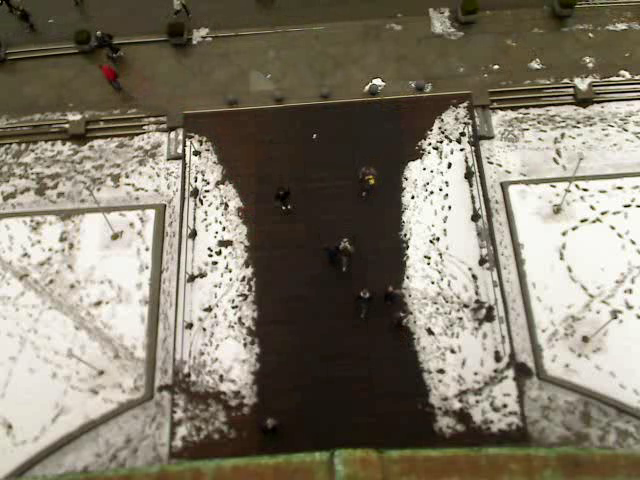
\includegraphics[keepaspectratio, scale=0.133]{images/eth.png}
    \caption{ETH}
    \label{Fig:datasets1}
  \end{subfigure}
  \hfill
  \begin{subfigure}{0.24\textwidth}
    \centering
    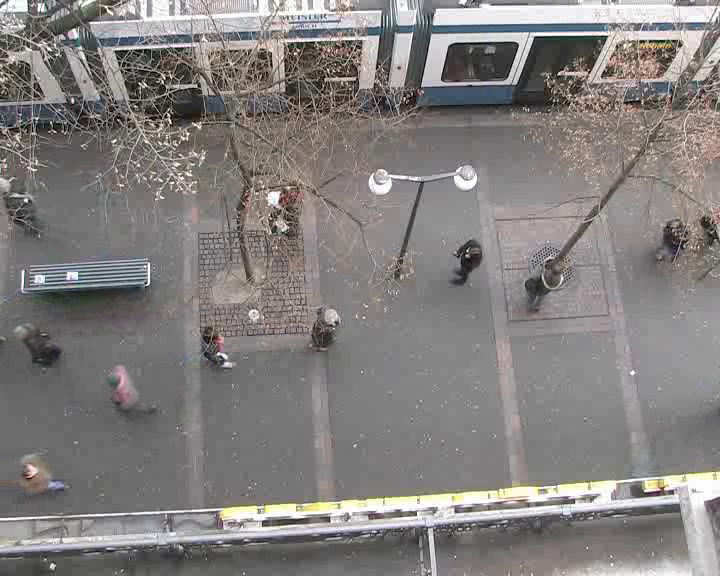
\includegraphics[keepaspectratio, scale=0.11]{images/hotel.png}
    \caption{HOTEL}
    \label{Fig:datasets2}
  \end{subfigure}
  \hfill
  \begin{subfigure}{0.24\textwidth}
    \centering
    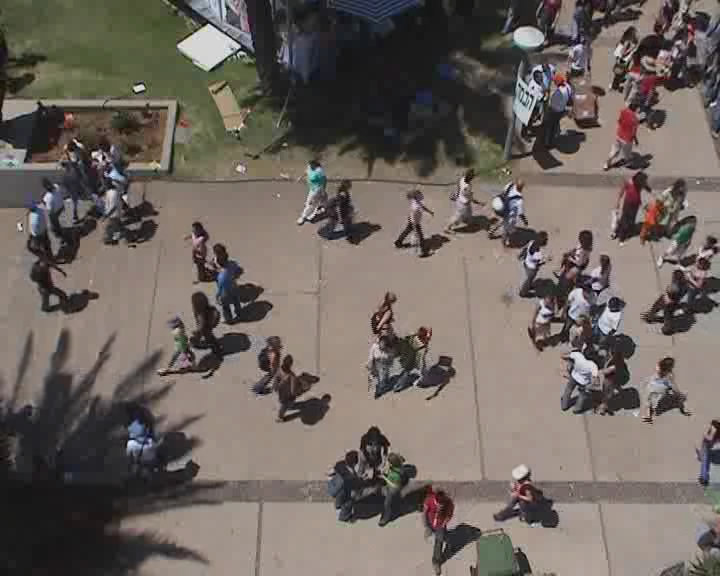
\includegraphics[keepaspectratio, scale=0.11]{images/students_003.jpg}
    \caption{UNIV}
    \label{Fig:datasets3}
  \end{subfigure}
  \hfill
  \begin{subfigure}{0.24\textwidth}
    \centering
    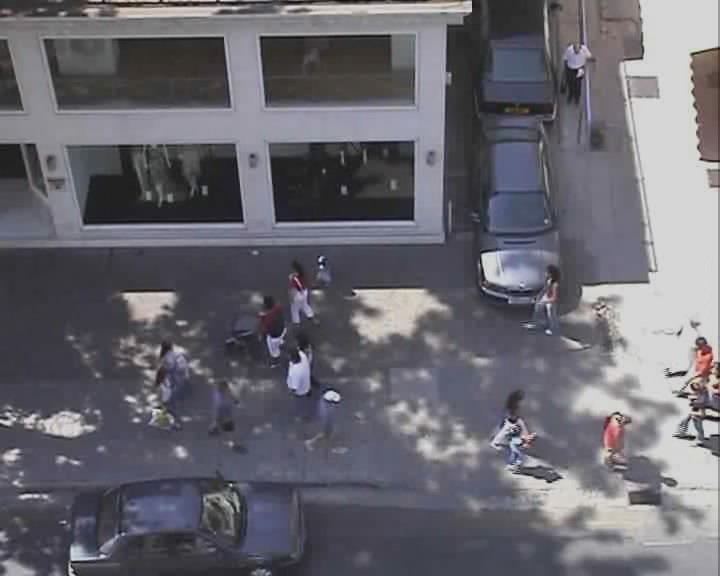
\includegraphics[keepaspectratio, scale=0.11]{images/crowds_zara01.jpg}
    \caption{ZARA1/ZARA2}
    \label{Fig:datasets4}
  \end{subfigure}
  \vspace{-8pt}
   \caption{Dataset examples}
  \label{Fig:datasets}
\end{figure}

\newpage

\section{学習環境}
本研究で行う学習は全て以下の\tabref{tab:environment}に示す環境で実施する.

\begin{table}[hbtp]
  \centering
  \caption{Experimental Setup}
  \label{tab:environment}
  \begin{tabular}{ll}
    \hline
    OS & Ubuntu 20.04.6 LTS \\
    CPU & Intel Core i7-10700F \\
    GPU & NVIDIA GeForce RTX 3060 \\
    Memory & 32GB \\
    Language & Python 3.8.10 \\
    Flamework & PyTorch 2.4.1 \\
    \hline
  \end{tabular}
\end{table}

\section{ネットワークの予備実験}
ロボットの行動を考慮した軌道予測を実験で確認する前に,まず提案したネットワークの基本的な性能を確認するため,予備実験を行った.

\subsection{実験概要}
本実験では,Mohamedら\cite{s-stgcnn}の実験方法に倣って,事前に学習したモデルを後述する2種類の指標で評価する.その結果を複数のベースラインモデルと比較し,提案ネットワークの性能を確認する.

\subsection{学習条件}
ネットワークの学習には,先行研究\cite{s-lstm,s-stgcnn}と同様にリーブワンアウト(Leave One Out)方式を採用することで,データセットを最大限に活用することができる.
具体的には,5つのシーンのうち1つをテストデータとして除外し,残り4つのシーンを用いてモデルの訓練と検証をする.テスト時には,8ステップにあたる3.2秒間観測し,次の12ステップにあたる4.8秒間の歩行者の将来位置を予測する.学習パラメータとしては,バッチサイズを128,オプティマイザにAdam\cite{kingma2014adam}を用い,学習率は$1e^{-3}$に設定した.最大エポック数は250とし,この条件下でネットワークを学習した.

\subsection{評価指標}
モデルの評価には,以下の2つの指標を用いた.

\begin{itemize}
  \item \textbf{ADE(Average Displacement Error)}\cite{pellegrini2009you-eth}:
    \begin{align}
      \text{ADE} = \frac{1}{TN} \sum_{t=1}^{T} \sum_{i=1}^{N} \| p^i_t - \hat{p}^i_t \|_2
    \end{align}
    ここで,$p^i_t$ は時刻 $t$ における歩行者 $i$ の実際の位置,$\hat{p}^i_t$ は予測された位置,$N$ は歩行者の総数,$T$ は予測の総時間ステップ数である.本研究では$T = 12$である.\figref{fig:ade}に示すように,ADEは実際の位置と予測位置の平均的な距離誤差を示す.
    \\
    \item \textbf{FDE(Final Displacement Error)}\cite{s-lstm}:
    \begin{align}
      \text{FDE} = \frac{1}{N} \sum_{i=1}^{N} \| p^i_t - \hat{p}^i_t \|_2 , \ t = t_{pred}
    \end{align}
    ここで,$p^i_t$ は最終時刻 $t_{pred}$ における歩行者 $i$ の実際の位置,$\hat{p}^i_t$ は予測された位置である.\figref{fig:fde}に示すように,FDEは予測の最終時刻における実際の位置と予測位置の距離誤差を示す.
\end{itemize}

\begin{figure}[hbtp]
  \centering
  \begin{minipage}{0.49\textwidth}
    \centering
    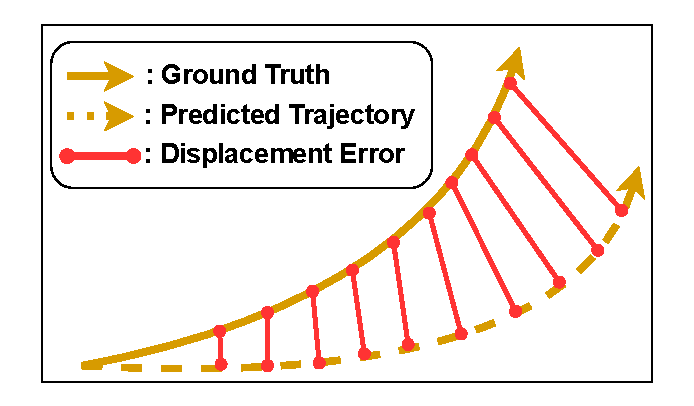
\includegraphics[width=\textwidth]{images/ade.pdf}
    \caption{ADE}
    \label{fig:ade}
  \end{minipage}
  \hfill
  \begin{minipage}{0.49\textwidth}
    \centering
    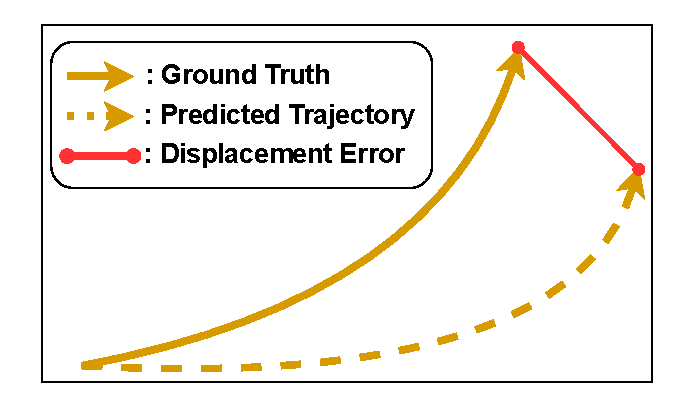
\includegraphics[width=\textwidth]{images/fde.pdf}
    \caption{FDE}
    \label{fig:fde}
  \end{minipage}
\end{figure}

\newpage

\subsection{結果と考察}
\begin{table}[hbtp]
  \centering
  \caption{Comparison of ADE/FDE for each model\protect\footnotemark[6]}
  \label{tab:val-results}
  \footnotesize
  \begin{tabular}{c||c|c|c|c|c|c}
  Model & ETH & HOTEL & UNIV & ZARA1 & ZARA2 & Average \\
  \hline \hline
  Linear \cite{s-lstm} & 1.33/2.94 & 0.39/0.72 & 0.82/1.59 & 0.62/1.21 & 0.77/1.42 & 0.79/1.59 \\
  \hline
  SR-LSTM-2 \cite{sr-lstm} & 0.63/1.25 & 0.37/0.74 & 0.51/1.10 & 0.41/0.90 & 0.32/0.70 & 0.45/0.94 \\
  \hline
  S-LSTM \cite{s-lstm} & 1.09/2.35 & 0.79/1.76 & 0.67/1.40 & 0.47/1.00 & 0.56/1.17 & 0.72/1.54 \\
  \hline
  S-GAN-P \cite{gupta2018social-s-gan-p} & 0.87/1.62 & 0.67/1.52 & 0.76/1.52 & 0.35/0.68 & 0.42/0.84 & 0.61/1.21 \\
  \hline
  SoPhie \cite{sadeghian2019sophie} & 0.70/1.43 & 0.76/1.67 & 0.54/1.24 & 0.30/0.63 & 0.38/0.78 & 0.54/1.15 \\
  \hline
  CGNS \cite{li2019conditional-cgns} & \textbf{0.62}/1.40 & 0.70/0.93 & 0.48/1.20 & 0.32/0.59 & 0.35/0.71 & 0.49/0.97 \\
  \hline
  PIF \cite{liang2019peeking-pif} & 0.73/1.65 & \textbf{0.30}/0.59 & 0.60/1.27 & 0.38/0.81 & 0.31/0.68 & 0.46/1.00 \\
  \hline
  STSGN \cite{zhang2019stochastic-stsgn} & 0.75/1.63 & 0.63/1.40 & 0.48/1.08 & 0.30/0.65 & \textbf{0.26}/0.57 & 0.48/0.99 \\
  \hline
  GAT \cite{s-bigat} & 0.68/1.29 & 0.68/1.40 & 0.57/1.29 & \textbf{0.29}/0.60 & 0.37/0.75 & 0.52/1.07 \\
  \hline
  Social-BIGAT \cite{s-bigat} & 0.69/1.29 & 0.49/1.01 & 0.55/1.32 & 0.30/0.62 & 0.36/0.75 & 0.48/1.00 \\
  \hline
  Social-STGCNN\cite{s-stgcnn} & 0.64/\textbf{1.11} & 0.49/0.85 & 0.44/0.79 & 0.34/0.53 & 0.30/0.48 & 0.44/0.75 \\
  \hline \hline
  \textbf{ours} & 0.69/1.24 & 0.33/\textbf{0.52} & \textbf{0.42}/\textbf{0.78} & \textbf{0.29}/\textbf{0.49} & \textbf{0.26}/\textbf{0.45} & \textbf{0.40}/\textbf{0.69} \\
  \hline
  \end{tabular}
\end{table}

\protect\footnotetext[6]{\cite{s-stgcnn}のデータを基に作成}

\tabref{tab:val-results}に示すように,本手法のモデルは2つの指標において他のベースラインモデルを上回る結果を示した.
平均ADEは0.40であり,最良のベースラインモデルと比較して約9%の改善を示した.また,FDEにおいても約8%の誤差減少が確認できた.
\tabref{tab:density}に示すとおり,5つのシーンのうちHOTEL,ZARA1,ZARA2は歩行者密度が低く,歩行者同士の複雑な相互作用が比較的少ないため,ADEとFDEの値は他のシーンよりも小さくなると考えられる.一方,
ETHとUNIVは歩行者密度が高く,複雑な相互作用が多いため,ADEとFDEの値が相対的に大きくなる傾向が見られた.

\vspace{30pt}
\begin{center}
  -----
  ここに具体的なネットワークの構造について言及している考察を追加
  -----
\end{center}

\newpage

\tabref{tab:param-results}は,各モデルのサイズと推論時間を本手法のモデルと比較したものである.
Social-STGCNN\cite{s-stgcnn}を除き,他のベースラインモデルと比較して,本手法のモデルはパラメータ数および推論時間の両方において効率的であることが分かる.
しかし,本手法のモデルのパラメータ数は28.6Kと,Social-STGCNNの約3倍に増加しており,推論時間も約20倍ほど遅くなっている.移動ロボットのナビゲーションにおいては実時間性が重要となるが,本研究のタスクでは0.4秒以内に予測が完了すれば十分なため,この推論時間の増加は実用上大きな問題にはならないと言える.

\begin{table}[hbtp]
  \begin{center}
  \caption{Number of samples and density of each dataset\protect\footnotemark[7]}
  \label{tab:density}
  % \footnotesize
  \begin{tabular}{c||c|c}
  Scene & Number of pedestrians & density [person$/ m^2$] \\ 
  \hline \hline
  ETH      & 358       & 8                      \\
  \hline
  HOTEL    & 389       & 5                      \\
  \hline
  UCY      & 434       & 8                      \\
  \hline
  ZARA1   & 148       & 4                      \\
  \hline
  ZARA2   & 204       & 5                      \\
  \hline
  \end{tabular}
  \end{center}
\end{table}

\protect\footnotetext[7]{\cite{箕浦大晃2022deep-survey}のデータを基に作成}

\begin{table}[hbtp]
  \centering
  \caption{Number of parameters and inference time for each model\protect\footnotemark[6]}
  \label{tab:param-results}
  % \footnotesize
  \begin{tabular}{c||c|c}
   & Parameters count & Inference time \\
  \hline\hline
  S-LSTM \cite{s-lstm} & 264K {\color{blue}(9.2x)} & 1.1789 {\color{blue}(27.4x)} \\
  \hline
  SR-LSTM-2 \cite{sr-lstm} & 64.9K {\color{blue}(2.3x)} & 0.1578 {\color{blue}(3.7x)} \\
  \hline
  S-GAN-P \cite{gupta2018social-s-gan-p} & 46.3K {\color{blue}(1.6x)} & 0.0968 {\color{blue}(2.3x)} \\
  \hline
  PIF \cite{liang2019peeking-pif} & 360.3K {\color{blue}(12.6x)} & 0.1145 {\color{blue}(2.7x)} \\
  \hline
  Social-STGCNN \cite{s-stgcnn} & \textbf{7.6K} {\color{blue}(0.3x)} & \textbf{0.0020} {\color{blue}(0.05x)} \\
  \hline \hline
  \textbf{ours} & 28.6K & 0.043 \\
  \hline 
  \end{tabular}
\end{table}

\protect\footnotetext[6]{\cite{s-stgcnn}のデータを基に作成}

\newpage
